\section{Tests}

\subsection{Current test of photo diode}
This test was done in order to dimension the resistor for the operational amplifier (op-amp), for the amplification.
The desired range of the output of the amplifier is 0 to 3.3 V to make it directly correlated with the ADC, which is powered by 3.3 V. 
\subsubsection{Setup}
The photo diode is put in a breadboard and the current through is measured using a multi meter. The different colored LED's are set up with a resistor so that they draw 50 mA of current which is the max DC-current\footnote{Ref to Application note}. The LED's and the photo diode are placed as they would on the final board, with a slight tilt towards the photo diode. A brick is then held over the diodes, and the current is read off the multi meter.
The setup can be seen in figure \ref{fig:photo_diode_current_setup}.

\begin{figure}[h]
 \centering
  \begin{circuitikz}
  \node[ground,name=gnd] at (0,0) {}; 
  \draw
  (gnd) to ++(0,1) to[ammeter] ++(2,0) to[pD] ++(2,0) to[R] ++(2,0)  |- (gnd)
  ;
  \draw (0,2) node[left] {$12V$} to[short, o-] ++(2,0) to[leD,mirror] ++(2,0) to[R] ++(2,0) |- (gnd); 
  \end{circuitikz}
  \caption{Setup to measure current of photo diode.}
  \label{fig:photo_diode_current_setup}
\end{figure}

\subsubsection{Results}
The results of the test can be seen in table \ref{tab::test_pd}.
\begin{table}[H]
\centering
 \begin{tabular}{|c|ccc|}
 \hline
 \diagbox{LED}{Brick}
        & Red         & Green       & Blue          \\ \hline
  Red   & $16\ \mu A$ & $2\ \mu A$  & $5\ \mu A$    \\ 
  Green & $5\ \mu A$  & $13\ \mu A$ & $9\ \mu A$    \\
  Blue  & $5\ \mu A$  & $6\ \mu A$  & $19\ \mu A$   \\
  \hline
 \end{tabular}
\caption{Outcome of the test}
\label{tab::test_pd}
\end{table}

Dividing $1 V$ with $10 \mu A$ in order to get the order of magnitude, gives $100 000$. This leads to the value of the resistor should be $100 k\Omega$.
This was tested to be accurate with the setup in figure \ref{fig:photo_diode_voltage_setup}.


\subsubsection{Conclusion}
Given the results of the test, and the fact that the current used here is lower than the one used in the project\footnote{Ref to section with LED circuit} it was decided that a value of $100 k\Omega$ would be a reasonable. This gives $0.1 \frac{V}{\mu A}$.

\subsection{Rise time test of amplifier} \label{sec:rise_time_test}

To test the rise time of the amplifier, the photo diode is set up as shown in figure \ref{fig:photo_diode_voltage_setup}.
It is expected that the load of the op-amp is not an ideal resistance. 
Due to the fact that we are not dealing with an ideal op-amp and the circuit introduces capacitance, the amplifier has a capacitive load. 
The feedback resistor is large enough so the circuit can be simplified by reducing it to a RC circuit.
A capacitor will always try to minimize the change in voltage, so with a high frequency of switching, the voltage will oscillate. To test the extend of this oscillation, a test setup without compensation is created.

\begin{wrapfigure}{r}{0.49\linewidth}
 \centering
  \begin{circuitikz}[scale=\figscale, every node/.style={scale=\figscale}]
  %opamp part
  \node[op amp,name=G] at (0,0) {}; 
  \node[ground,name=gnd] at ($(G.+)+(-3,-1)$) {}; 
  \draw
  (gnd) -| (G.+) 
  (gnd) to[short] ($(G.-)+(-3,0)$) to[pD] ($(G.-)+(-0.5,0)$) node[name=intersection] {} to (G.-)
  (G.out) to ++(0,1.5) coordinate(Rright) to[R=$100K\Omega$] ++(-2.7,0)  -| (intersection.center) coordinate(Rleft)
  (G.out) to[short,-o] ++(1,0) node[right,name=out] {$V_{out}$} 
  (out.west) to[voltmeter] ++(0,-1.5) -| (gnd) 
  ;
  \draw (Rleft) |- ++(1,2) to[C=$C_f$] ++(1,0) -| (Rright);
  %led part
  \node[nmos, name=mosfet,rotate=-90] at (-3,3.5) {};
  \draw (mosfet.S) -| (gnd) 
  (mosfet.D) to[leD] ++(2,0) to[R=$160\Omega$] ++(2,0) to[short,-o] ++(1,0) node[right] {$12 V$}
  (gnd) |- ($(mosfet.G)+(0,1)$) to[sqV] (mosfet.G) 
  ;
  \end{circuitikz}
  \caption{Setup to measure voltage of photo diode.}
  \label{fig:photo_diode_voltage_setup}
 \end{wrapfigure}

A red diode was used for the test, so the expected output voltage is $2 V$.
To test for ringing effect, the naive setup, shown in figure \ref{fig:photo_diode_voltage_setup}, 
is used to see if the op-amp can keep up with a high speed signal. The capacitance, $C_f$ is removed.\
This resulted in a ringing effect and thus the signal could not settle before the diode is turned off again.
In figure \ref{fig::scope_op_amp_no_C} can this effect be seen.


To avoid the ringing effect, a capacitor is added as seen in figure \ref{fig:photo_diode_voltage_setup}.
To find a proper capacitance, equation \ref{eq:capacitance_approximate}
\footnote{Practical Techniques to Avoid Instability due to capacitive load, p2}
is used to find an approximate.
The frequency, $f$, is found by measuring the period on the naive signal.
The period was found to be between $6$ and $7$ $\mu S$.
The capacitance estimate is thus between $9.55$ and $11.1 pf$. 
A feedback capacitor of $10 pf$ was chosen.

\begin{equation}
 C_f = \frac{1}{2 \pi f R_f} \label{eq:capacitance_approximate}
\end{equation}

In figure \ref{fig::scope_op_amp_with_C}, it can be seen that the amplifier now is critically damped and thus able to settle at a higher frequency.
The signal must be settled in the time the ADC measures, which is $560 ns$ from the falling edge of the chip select.
As it can be seen, the signal is readable at $65 kHz$.

\begin{figure}[h]
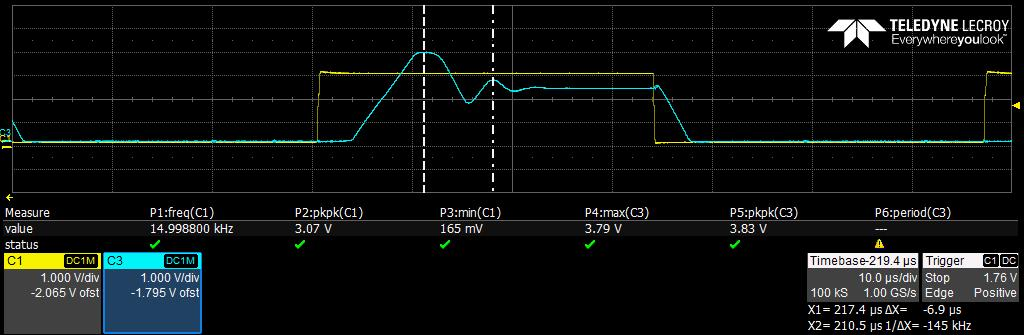
\includegraphics[width=0.9\linewidth]{img/amp_test_ringing1.jpg}
\caption{Ringing effect of amplifier. The yellow line shows when the LED is turned on and off, and the blue is the output of the amplifier}
\label{fig::scope_op_amp_no_C}
\end{figure}


\begin{figure}[h]
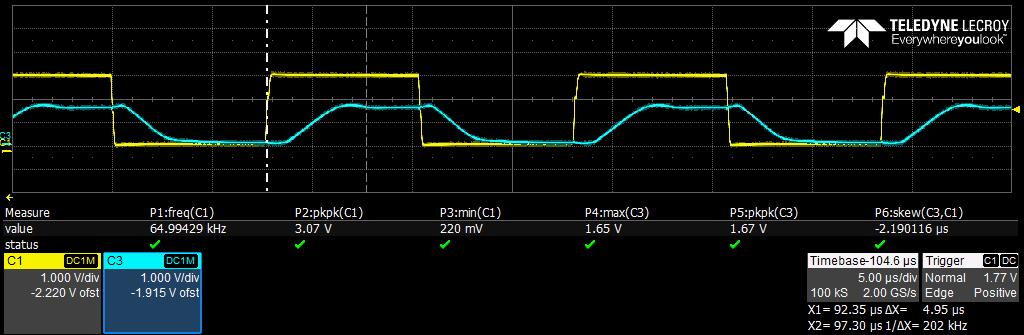
\includegraphics[width=0.9\linewidth]{img/ringing_test_filtered_rise.jpg}
\caption{Ringing effect of amplifier. The yellow line shows when the LED is turned on and off, and the blue is the output of the amplifier}
\label{fig::scope_op_amp_with_C}
\end{figure}

\subsection{ADC}
To test if the ADC works with the FPGA, the ADC was tested on a breadboard.
A controlled input was given to the ADC and the MISO signal was analyzed to find the ADC value.
The ADC value is a the last 10 bits of the 17 bit package on the MISO, sent after a falling edge on the CS.
In figure \ref{fig:scope_adc} is the oscilloscope readings for a test with 2.1 V input shown.

To see how the ADC handles the input voltage a series of measurements has been made with a 0.1 V step between measurements.
Figure \ref{fig:adc_values} shows the ADC values in decimal in relation to the input voltage.
From this it can be seen that the ADC values are proportional to the input voltage and thus the ADC communication works.
The data code for the data processing can be found in appendix \ref{app:adc_R_code}.

\begin{figure}[h]
 \centering
 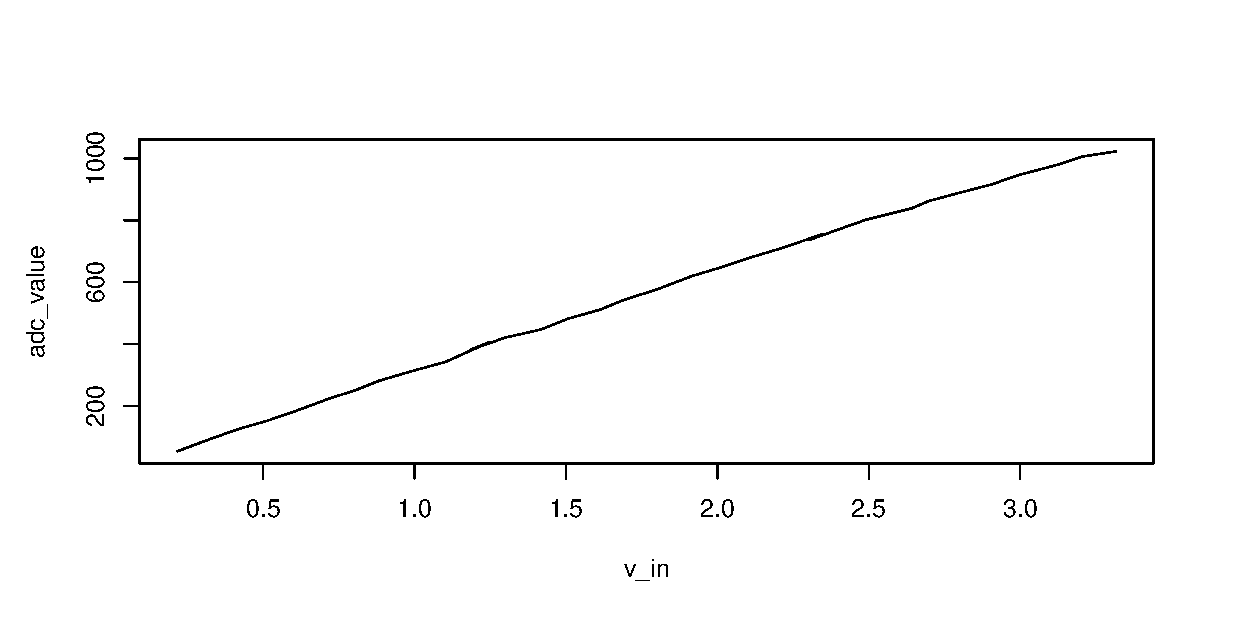
\includegraphics[width=0.7\textwidth]{img/ADC_values}
 \caption{ADC values in relation to input voltage.}
 \label{fig:adc_values}
\end{figure}

\begin{figure}[h]
    \centering
    \begin{tikzpicture}
        \node {
        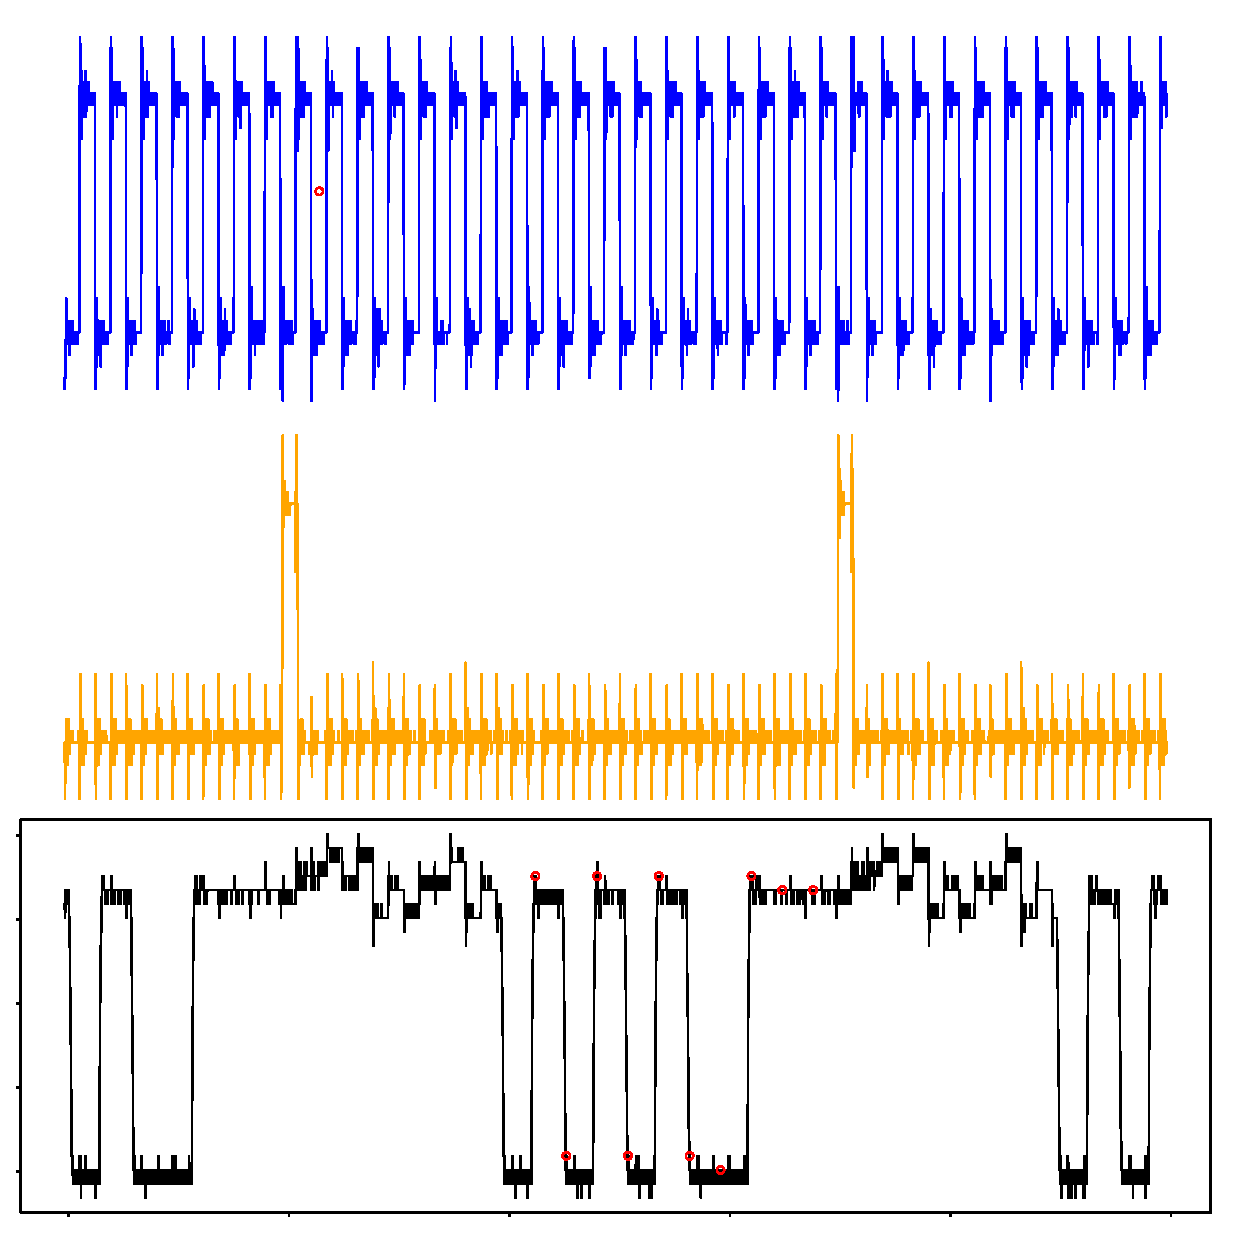
\includegraphics[width=0.7\textwidth]{img/scope_adc} 
        };
        \node at (-6.5,4)  {CLK};
        \node at (-6.5,0)  {CS};
        \node at (-6.5,-4) {MISO};
    \end{tikzpicture}
    \caption[Oscilloscope measurements for ADC]
            {Oscilloscope output of the ADC connections for the 2.107 V RMS input. The red dots signify when the signal is read.}
            \label{fig:scope_adc}
\end{figure}

% the figures I like is BACK
\begin{figure}[h]
\centering
\begin{tikztimingtable}[xscale=0.3]
 slow\_clk       & L2{26{2{T}}          }L\\
 led\_signal     & Z 1{50D{R}}1{2Z} 1{50D{G}}1{2Z}      L\\
 adc\_read       & L2{13{2L}2{2H}11{2L} }L\\
 adc\_transfer   & L2{15{2L}10{2H}1{2L} }L\\
 signal\_complete& L2{25{2L}1{2H}       }L\\
\end{tikztimingtable}
 \caption{ADC communication, naive approach.}\label{fig:naive_communication}
\end{figure}

\begin{figure}[h]
\centering
\begin{tikztimingtable}[xscale=0.3]
 slow\_clk       & L12{2{T}}3{19{2{T}}          }\\
 led\_signal     & Z 1{38D{R}} 1{38D{G}}1{38D{B}} 1{24D{R}} \\
 adc\_read       & L12{2L} 3{5{2L}2{2H}11{2L}1{2L} }\\
 adc\_transfer   & L12{2L} 3{7{2L}1{20D{adc}}1{2L}1{2L} }\\ 
 sample\_done    & L29{2L} 2{1{2H}16{2L}     2{2L} }1{2H}LL\\ 
 \extracode
    \vertlines[dashed]{61,77,99,115} %8 clock cycles
\end{tikztimingtable}
\caption{ADC communication optimized.}\label{fig:optimized_communication}
\end{figure}